%\documentclass{article}
%\usepackage{graphicx,subfigure}
%\begin{document}

\begin{figure}[!h]
  \centering
  \subfigure[Photograph showing a three Merino wool staples representing (left to right) the {\em unaligned}, {\em stretched}, and {\em unfolded} staple crimp types.]{
    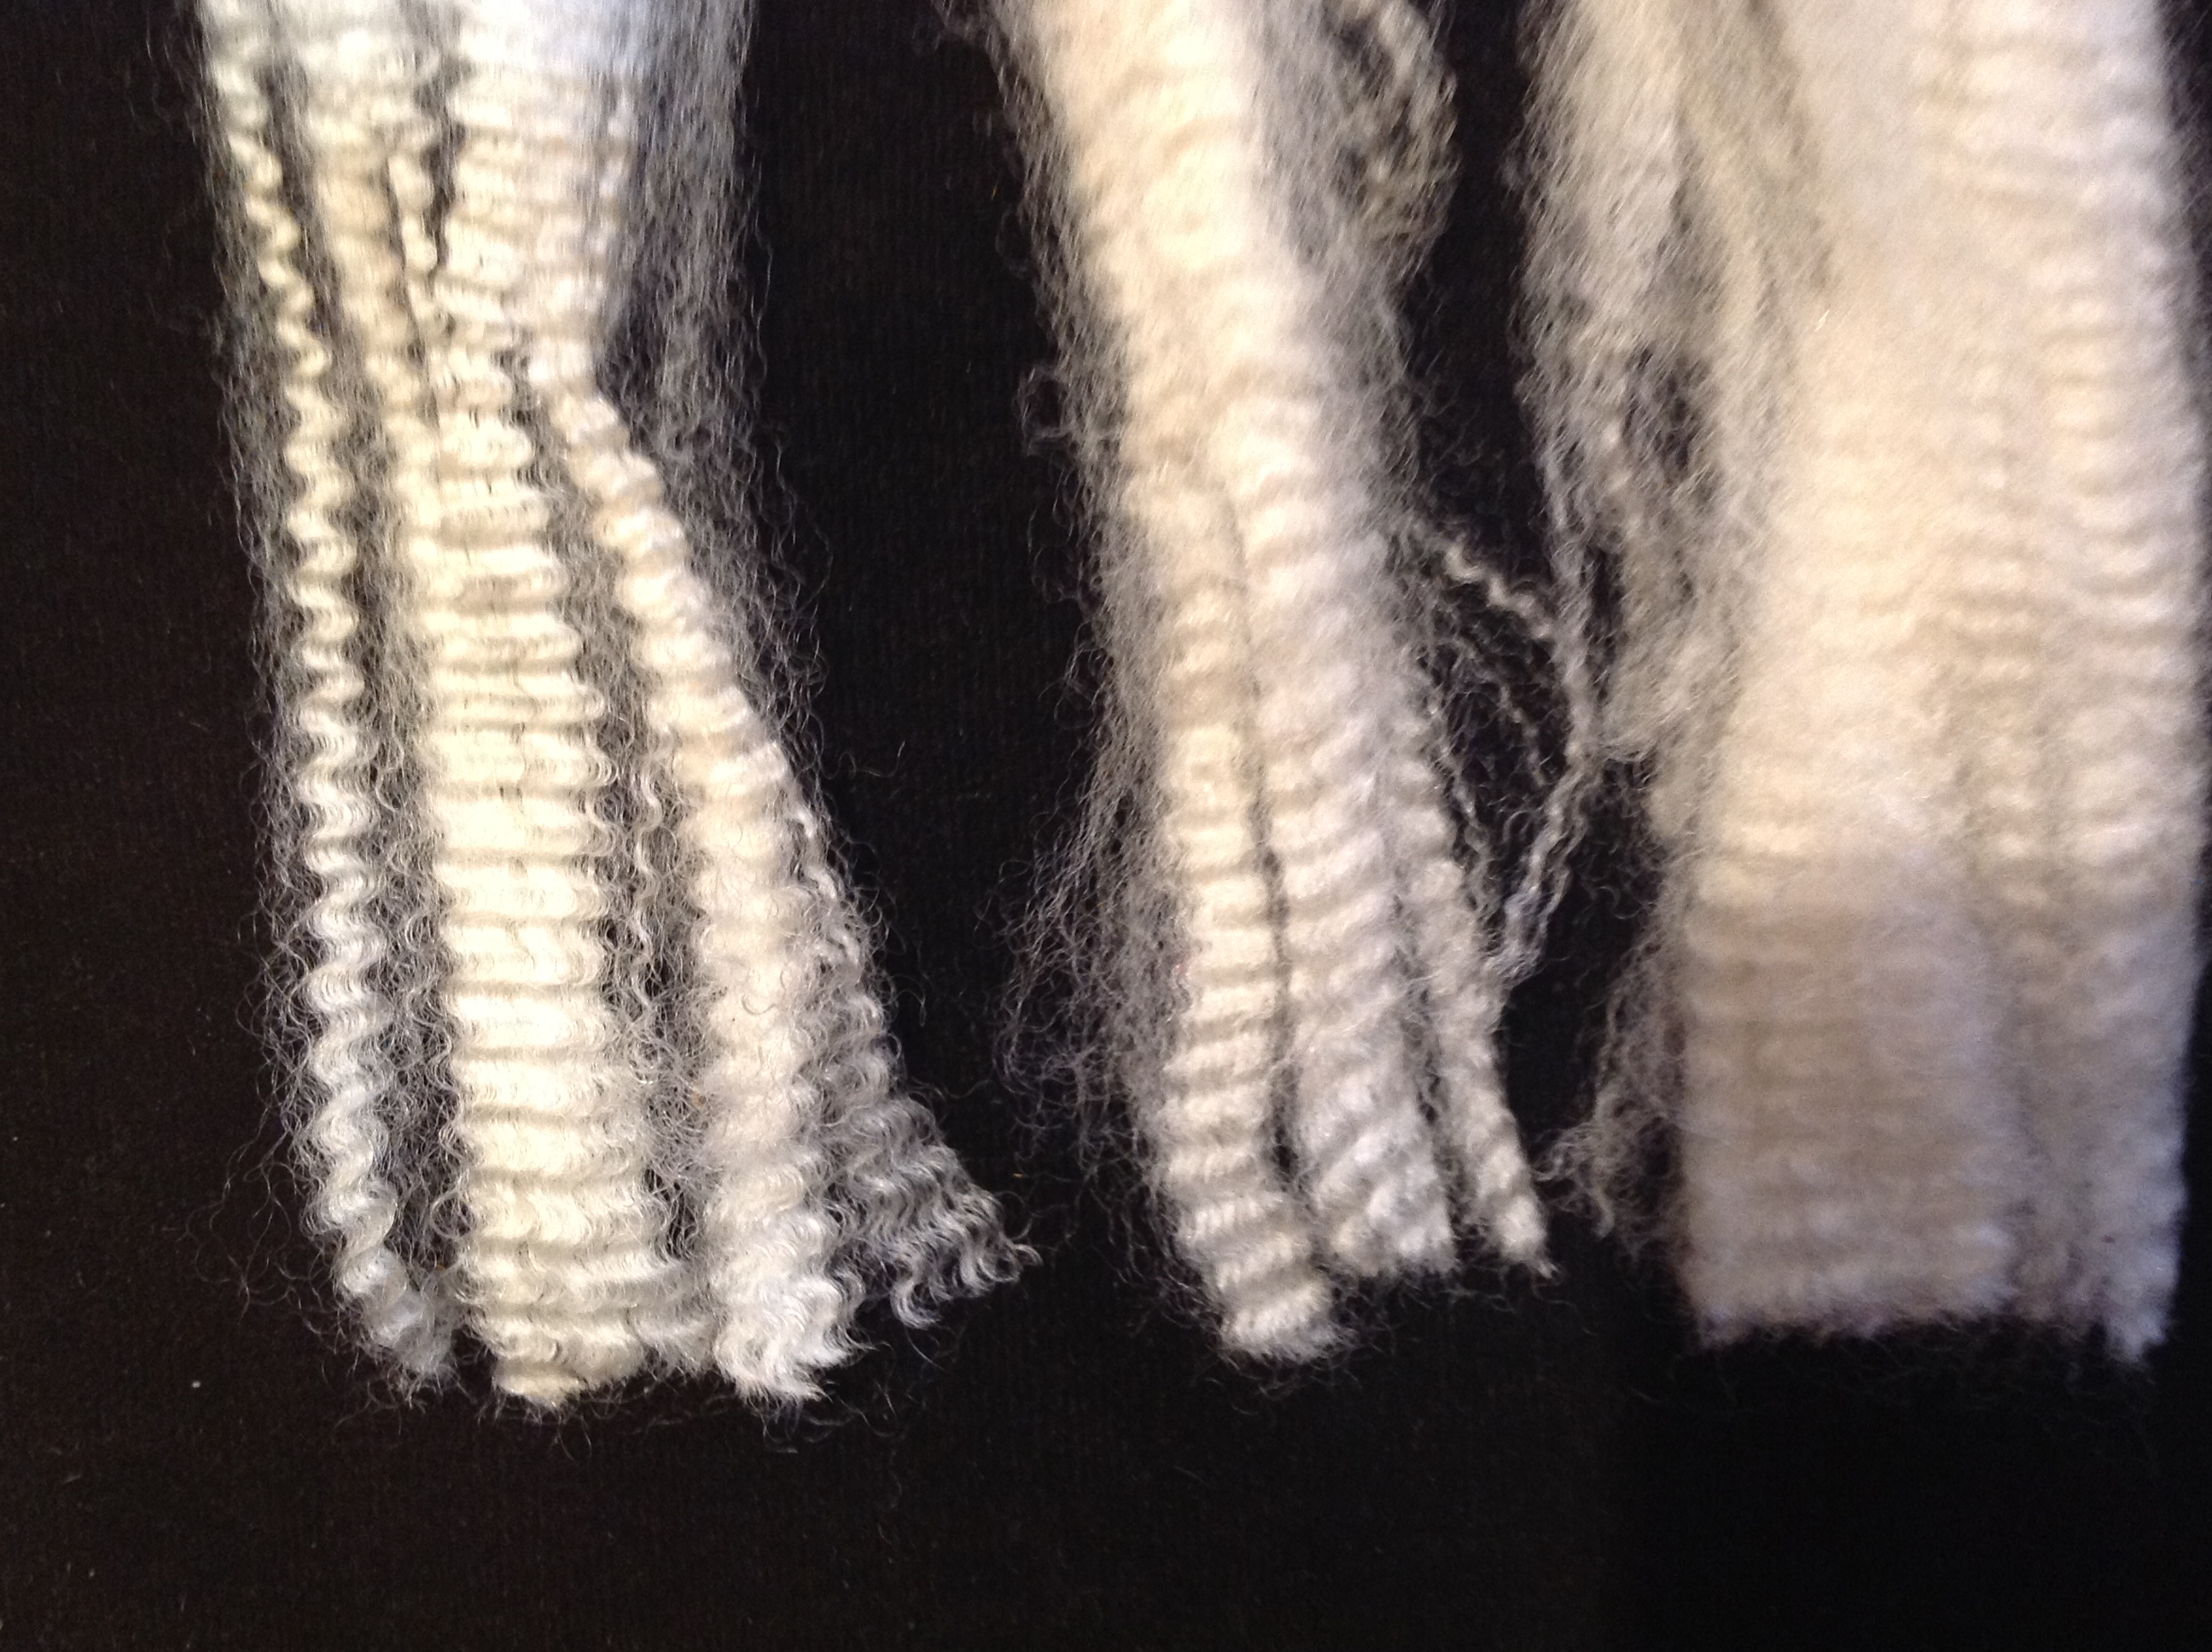
\includegraphics[width=1.0\textwidth,angle=180]{figwoolphoto.jpg}
%   photo549.499.525.jpg is original photo 
%   \caption{Photograph showing a three Merino wool staples representing (left to right) the {\em unaligned}, {\em stretched}, and {\em unfolded} staple crimp types.  photo549.499.525.jpg}
    \label{fig:woolphoto}
  }



  \subfigure[Photomicrographs showing multiple bundles of fibres for each of the three staple crimp types. Left to right {\em unaligned}, {\em stretched}, and {\em unfolded}.]{
    \includegraphics[width=1.0\textwidth]{figthreetypes.jpg}
%   composite of unalfib549.jpg, strebun574.jpg, unfobun.jpg
%   \caption{Photomicrographs showing multiple bundles of fibres for each of the three staple crimp types shown in Figure~\ref{fig:woolphoto}. Left to right {\em unaligned}, {\em stretched}, and {\em unfolded}.  composite of unalfib549.jpg, strebun574.jpg, unfobun.jpg}
    \label{fig:threetypes}
  }
 
  \caption{Definition of three Merino staple crimp types. Left to right {\em unaligned}, {\em stretched}, and {\em unfolded}.}
  \label{fig:woolphot3types}

\end{figure}

%\end{document}

